\chapter{Achtergrond}


\section{Displacement pipetten}
\subsection{Air-Displacement}
Bij Air-Displacement pipetten wordt er geen direct contatct gemaakt tussen de vloeistof en de zuiger. Er is een laag lucht die tussen de vloeistof en de zuiger zit. Dit zorgt ervoor dat er geen contaminatie van de vloeistof kan optreden. Dit is een belangrijk voordeel. Er wordt echter wel aan nauwkeurigheid ingeboet. Dit komt door de aanwezigheid van zowel luchtdrukverschijnselen als opervlaktespanningen in de vloeistof. Deze fouten kunnen deels verholpen worden met correctieberkeningen zoals in\ \cite{RN15} of lookup-tabellen zoals in\ \cite{RN35}. Dit is echter niet altijd mogelijk. Bij het pipetteren van zeer kleine volumes kan de invloed van de oppervlaktespanning zo groot zijn dat er geen correctie meer mogelijk is. Dit komt doordat de oppervlaktespanning een grotere invloed heeft op de vloeistof dan de luchtdruk. Dit kan opgelost worden door gebruik te maken van een andere techniek, namelijk positive displacement zoals beschreven in\ \cite{RN15}.
\subsubsection{Theoretische achtergrond}
In\ \cite{RN15} staat beschreven hoe een air-displacement pipet werkt via de ideale gaswet. Er wordt een omgeving van lagere druk gecreëerd door het veranderen van het volume van de pipet. Dit volume wordt ingenomen door de vloeistof waar de pipetpunt zich in bevindt. Bij een mondpipet wordt deze negatieve druk gecreëerd door de longen van de operator. Bij de mechanische pipet wordt deze via de peer gecreëerd door deze initieel in te drukken en daarna terug te laten opvullen.
\subsection{Positive Displacement}
Positive displacement pipetten zijn een alternatieve oplossing waarbij er wel contact is tussen de vloeistof en de zuiger. Er treden dus geen oppervlaktespanningen op aangezien de vloeistof overal contact maakt met de zuiger. Dit heeft voordelen op vlak van precisie. Vooral bij vloeistoffen die sterk verschillen van water. Zo worden positive displacement pipetten in \ \cite{RN37} voorgesteld als methode om cel-cultuur-media of BSA te pipetteren. Ze dragen echter een groter risico op contaminatie, al kan dit wel verholpen worden.

\section{Pipette types}
\subsection{Mondpipetten}
Mondpipetten waren doorheen de 19e en in het begin van de 20e eeuw de standaard voor het pipetteren. De operator zorgde hier zelf voor een negatieve druk door in te ademen. Dit was enkel mogelijk als air-displacement pipet. In\ \cite{RN21} wordt bijvoorbeeld een ontwerp voor een mondpipet voorgesteld om steriliteitstesten mee uit te voeren. In 1950 werd door A. J. Swallow in\cite{RN18} de eerste mechanische pipet voorgesteld voor het pipetteren van radioactieve stoffen. Hierdoor was er geen contact mogelijk tussen de mond en de te pipetteren vloeistof. Dit helpt ook bij het vermijden van besmetting van labopersoneel zoals beschreven in\ \cite{RN20}.
\subsection{Analoge pipetten}\label{sec: Analoge pipetten}
Analoge pipetten, zoals beschreven in de patenten\ \cite{RN16} en\ \cite{RN17}, werken volgens het principe van een zuigermechanisme. Het instellen van het gewenste volume gebeurt door het aanpassen van de slag van de zuiger zoals te zien in \autoref{fig:werking US4744955} en \autoref{fig:werking US5320810}.
\\[12pt]In het geval van\ \cite{RN17} gebeurt dit via een instelwiel. Door het draaien aan dit wiel wordt een loodschroef axiaal verplaatst, wat de beginpositie van de zuigerstang aanpast. Bij een kleiner ingesteld volume zal de zuigerstang in rustpositie korter lijken. De zuigerstang kan vervolgens worden ingedrukt tot aan een vaste stopmoer, die steeds op dezelfde positie blijft. Omdat de beginpositie van de zuigerstang verschuift, verandert de totale slag van de zuiger, en daarmee het op te nemen volume.
\\[12pt]Het principe in\ \cite{RN16} is vergelijkbaar, maar eenvoudiger uitgevoerd. Hier wordt het volume ingesteld door het onderste deel van de pipet verder in te schroeven, waardoor de eindpositie van de zuiger wordt bepaald. Op die manier wordt ook de zuigerslag en dus het volume aangepast.
\\[12pt]De analoge pipetten beschreven in deze patenten gebruiken air-displacement maar deze pipetten kunnen ook met positive displacement gevonden worden. In geval van\ \cite{RN17} gebeurt dit met een zuiger (44) die relatief verder van de pipetteer-punt (28) staat dan bij\ \cite{RN16}.\ \cite{RN16} is eenvoudiger uitgevoerd dan\ \cite{RN17}. Er zijn minder dichtingen en er is geen display om het gewenste volume van af te lezen. Dit maakt echter ook dat\ \cite{RN16} meer problemen zal hebben op vlak van lekkage en dus precisie.
\\[12pt]\begin{minipage}[t]{0.49\textwidth}
    \vspace{0pt}
    \begin{figure}[H]
        \centering
        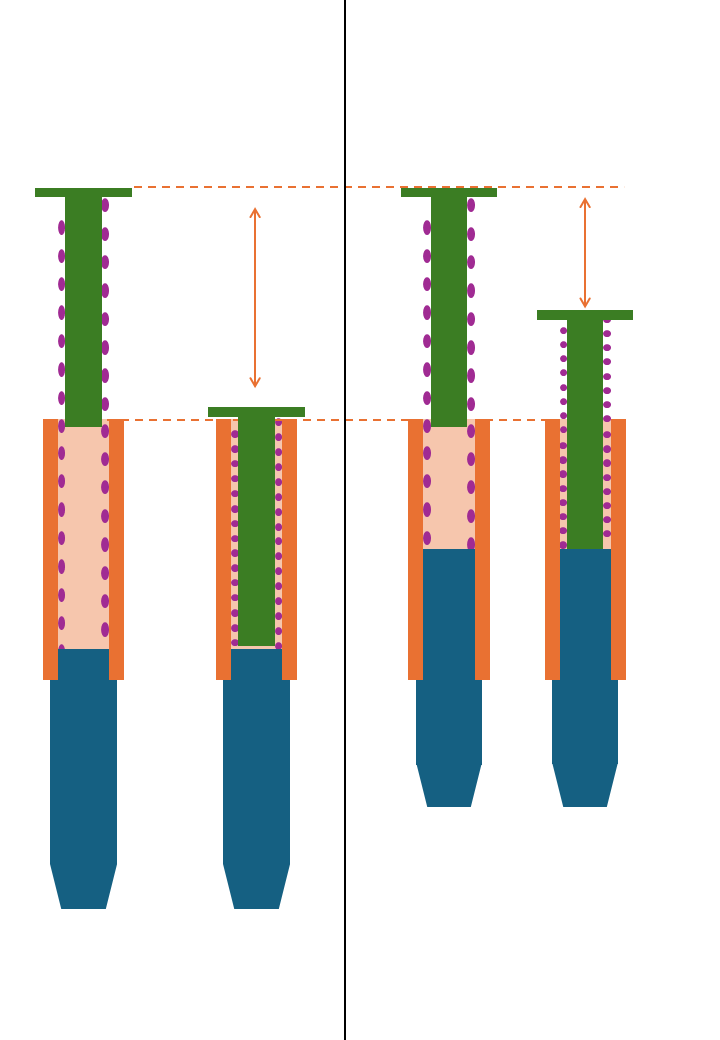
\includegraphics[height=7cm]{figures/Werking US4744955.png}
        \caption{US4744955.}\label{fig:werking US4744955}
        Gebaseerd op\ \cite{RN16}
    \end{figure}
\end{minipage}
\begin{minipage}[t]{0.49\textwidth}
    \vspace{0pt}
    \begin{figure}[H]
        \centering
        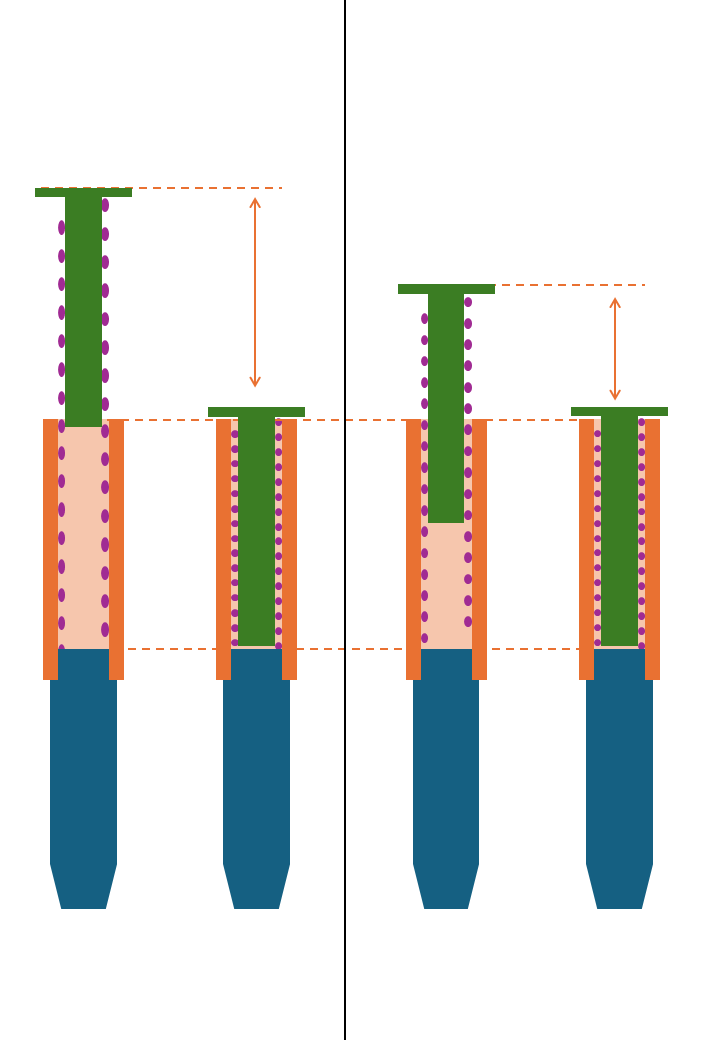
\includegraphics[height=7cm]{figures/Werking US5320810.png}
        \caption{US5320810.}\label{fig:werking US5320810}
        Gebaseerd op\ \cite{RN17}
    \end{figure}
\end{minipage}\\

\subsection{Elektronische pipetten}
Elektronische Pipetten bouwen verder op dezelfde principes als analoge pipetten. Bij elektronische pipetten wordt de actuatie van de zuiger motorisch aangedreven. Zo wordt dit in\ \cite{RN35} met een stappermotor gedaan. Dit laat toe om de zuiger met een hoge precisie te verplaatsen. Voor deze methode is de precisie van de motor cruciaal aangezien dit de maximale precisie van de pipet zal bepalen. In het eerder genoemde patent wordt hiervoor gebruik gemaakt van microstepping. Microstepping is een belangrijk voordeel van stappermotoren en laat toe om met een precisie van enkele tientalle nl te pipetteren. 
\\[12pt]De rotationele beweging van de motor moet omgezet worden tot een axiale beweging in de zuiger. In het geval van\ \cite{RN35} wordt dit met een loodschroef gedaan. Om te bepalen hoeveel stappen er voor een bepaald volume nodig zijn wordt er in het patent gebruik gemaakt van een lookup-tabel met empirisch bepaalde waarden. Ook is er een calibratietabel die deze waarden verfijnt naar de toepassing. Deze houdt mede rekening met oppervlaktespanningen en atmosferische invloeden. 
\\[12pt]In het geval van een stappermotor kan er ook een vergelijking afgeleid worden op basis van de lood van de schroef, de doorsnede van de zuiger en het aantal stappen per rotatie. Dit gaat echter uit van ideale omstandigheden zonder gemiste stappen en is dus niet realistisch. Gemiste stappen zijn dan ook een beperkende factor voor stappermotoren aangezien dit leidt tot fouten in het gepipeteerde volume.\ \cite{RN36} maakt gebruik van een senor om verplaatsing van de zuiger te bepalen. Dit maakt een closed-loop systeem met mogelijkheid tot regeling.